%%%%%%%%%%%%%%%%%%%%%%%%%%%%%%%%%%%%%%%%%%%%%%%%%%%%%%%%%%%%%%%%%%%%%%%%%%%%%%%%
%2345678901234567890123456789012345678901234567890123456789012345678901234567890
%        1         2         3         4         5         6         7         8

\documentclass[letterpaper, 10 pt, conference]{ieeeconf}  % Comment this line out
                                                          % if you need a4paper
%\documentclass[a4paper, 10pt, conference]{ieeeconf}      % Use this line for a4
                                                          % paper

\IEEEoverridecommandlockouts                              % This command is only
                                                          % needed if you want to
                                                          % use the \thanks command
\overrideIEEEmargins
% See the \addtolength command later in the file to balance the column lengths
% on the last page of the document

\usepackage[utf8]{inputenc}
\usepackage[T1]{fontenc}
\usepackage{graphicx}
\usepackage{amsmath}
\usepackage{listings}
% The following packages can be found on http:\\www.ctan.org
%\usepackage{graphics} % for pdf, bitmapped graphics files
%\usepackage{epsfig} % for postscript graphics files
%\usepackage{mathptmx} % assumes new font selection scheme installed
%\usepackage{mathptmx} % assumes new font selection scheme installed
%\usepackage{amsmath} % assumes amsmath package installed
%\usepackage{amssymb}  % assumes amsmath package installed

\title{\LARGE \bf
Análise de SpeedUp ao Paralelizar o Problema de Encriptação de Dados Baseado no Método \textit{Rail Fence Cipher}
}

%\author{ \parbox{3 in}{\centering Huibert Kwakernaak*
%         \thanks{*Use the $\backslash$thanks command to put information here}\\
%         Faculty of Electrical Engineering, Mathematics and Computer Science\\
%         University of Twente\\
%         7500 AE Enschede, The Netherlands\\
%         {\tt\small h.kwakernaak@autsubmit.com}}
%         \hspace*{ 0.5 in}
%         \parbox{3 in}{ \centering Pradeep Misra**
%         \thanks{**The footnote marks may be inserted manually}\\
%        Department of Electrical Engineering \\
%         Wright State University\\
%         Dayton, OH 45435, USA\\
%         {\tt\small pmisra@cs.wright.edu}}
%}

\author{Arthur Rodrigues Batista$^{1}$ e Douglas Ferreira Delefrati$^{2}$% <-this % stops a space
 \\Universidade Estadual de Maringá\\
   Departamento de informática\\
   Maringá, Paraná, Brasil
 \\ e-mail: ra105422@uem.br$^{1}$ | ra103654@uem.br$^{2}$
}


\begin{document}



\maketitle
\thispagestyle{empty}
\pagestyle{empty}


%%%%%%%%%%%%%%%%%%%%%%%%%%%%%%%%%%%%%%%%%%%%%%%%%%%%%%%%%%%%%%%%%%%%%%%%%%%%%%%%
\begin{abstract}

This article performs a quantitative analysis of the sequential and parallel performance of the Rail Fence Chipher cipher encryption algorithm. During the text, will be presented the sequential algorithm and the modifications that were made with the objective of obtaining a parallel implementation, whose performance has exceeded the sequential version. The results were positive, reaching a speedup from two to four hreads. After a specific size, provided as input, performance decreases due to limitations of the hardware on which the experiments were performed.

\end{abstract}

\begin{resumo}

Este artigo realiza uma análise quantitativa do desempenho sequencial e paralelo do algoritmo de criptografia de cifra \textit{Rail Fence Chipher}. Ao decorrer do texto, será apresentado o algoritmo sequencial e as modificações que foram feitas com o objetivo de obter uma implementação paralela, cujo desempenho tenha excedido à versão sequencial. Os resultados foram positivos, alcançando um \textit{speedup} de dois para quatro \textit{threads}. Após um tamanho específico, fornecido como entrada, o desempenho diminui em decorrência de limitações do hardware na qual os experimentos foram realizados.

\end{resumo}


%%%%%%%%%%%%%%%%%%%%%%%%%%%%%%%%%%%%%%%%%%%%%%%%%%%%%%%%%%%%%%%%%%%%%%%%%%%%%%%%
\section{Introdução}
A definição clássica de algoritmo é uma sequência finita de instruções não ambíguas com a finalidade de resolver uma classe de problemas. Tradicionalmente, os computadores foram projetados para executar os algoritmos de maneira sequencial, ou seja, uma instrução qualquer iniciaria após o término da instrução anterior. Entretanto, conforme a necessidade de mais processamento aumentou, novas estratégias foram sendo implementadas para suprir a demanda por processamento. Neste contexto, pesquisadores propuseram o conceito de paralelismo.

O paralelismo pode ser alcançado de diferentes formas, cada uma restrita pelos limites tecnológicos de sua época. A primeira tentativa de executar códigos de maneira paralela foi implementando a paralelização diretamente no hardware. Neste método, os processadores possuem um pipeline com $n$ etapas, possibilitando duas ou mais instruções serem executadas simultaneamente, explorando o potencial de sobreposição entre instruções de um código. Esse tipo de paralelismo melhorou consideravelmente o desempenho dos processadores, sendo utilizado até os dias atuais. Além disto, essa abordagem não modificou o modo como os desenvolvedores implementavam seus códigos, permitindo-lhes manter os mesmos paradigmas de programação por décadas.

No entanto, limitações físicas do hardware impossibilitam que o desempenho aumente exponencialmente como a lei de Moore \footnote{A Lei de Moore se refere à percepção de Moore de que o número de transistores em um microchip dobra a cada dois anos, embora o custo dos computadores seja reduzido pela metade. A Lei de Moore afirma que podemos esperar que a velocidade e a capacidade de nossos computadores aumentem exponencialmente} previa \cite{c6}. Sendo assim, novas estratégias foram pensadas para obter melhor performance. Uma delas foi a programação paralela utilizado múltiplas \textit{threads}, resumindo-se em distribuir, em duas ou mais processos, que podem se executadas paralelamente com o objetivo de reduzir o tempo de computação do problema como um todo.

Idealmente, se dividirmos um processo qualquer com tempo de execução $P$ em $T_{p}$ \textit{threads}, teríamos um ganho de performance linear \cite{c5}. Entretanto, existem diversas complicações intrínsecas à paralelização no código \cite{c2}, tais como o sincronismo, granularidade das tarefas e compartilhamento de memória entre as \textit{threads}. Todos esses problemas requerem processamento adicional do sistema operacional para manter a integridade do código, comumente chamado de \textit{overhead}.

Em detrimento do \textit{overhead}, a paralelização não é recomendada para todos os algoritmos, pois dependendo da classe do problema ou o tempo de execução, o desempenho pode piorar quando comparada à abordagem sequencial \cite{c5}. 

Isto posto, a proposta do presente trabalho foi avaliar o desempenho do paralelismo aplicado ao problema de criptografia de dados, com o intuito de estabelecer algumas constatações empíricas em relação às vantagens, assim como as limitações dessa estratégia. Para tal, foram realizadas uma série de experimentos. Dentre estes, avaliamos à performance à medida que o tamanho da entrada fosse variado, assim como a quantidade de \textit{threads}. A motivação em modificar esses parâmetros foi identificar o ponto limite de aprimoramento de \textit{speedup} utilizando o paralelismo, dadas às restrições da máquina.

Ao longo do restante dessa apresentação, daremos um enfoque relacionado à técnica de criptografia de dados baseado no modelo \textit{Rail Fence Cipher}. Além disso, apresentaremos uma solução paralela ao problema baseada em paralelismo de dados. Também será comentado mais a respeito das métricas de avaliação de performance de programas paralelos e as especificações dos experimentos, tais como a máquina utilizada assim como o tamanho das entradas.

Embora o resultado obtida tenha sido um maior \textit{speedup} ao passo que a entrada tenha transitada de \textit{Pequena} à \textit{Média}, devido às limitações do hardware, como quantidade de núcleos e capacidade da memória RAM, o desempenho da implementação paralela foi comprometido para a maior entrada. A explicação para tal se deve ao fato do tamanho dessa entrada ocasionar uma alta troca de dados do programa com o disco rígido, também conhecido por \textit{swap}, em que, devido à limitação da máquina, a partir de um determinado tamanho, aumenta-se substancialmente o tempo de execução do algoritmo.

\section{Trabalhos relacionados}
Algoritmos de encriptação do tipo cifra normalmente utilizam a representação de matrizes para estruturar os dados, isso pode criar diversas adversidades na implementação pois como já é conhecido,  operações de matrizes consomem tempo e espaço consideráveis. Algoritmos como \cite{c8} e \cite{c9} foram propostos para paralelizar a multiplicação de matrizes aumentando seu desempenho. Mais especificamente para algoritmos de cifra, existem diversos trabalhos como o \cite{c10} que propôs um método eficiente de geração de matriz auto-invertível para um algoritmo de cifra de Hill. Com isso, surgiram outras implementações utilizando esse algoritmo para obter um maior desempenho no algoritmo de cifra de Hill \cite{c7}. Essas implementações equilibram a comunicação entre processos, dependências e nível de paralelismo para maximizar a eficiência.

\section{Rail Fence Cipher}

\subsection{Formulação do Problema}
O Rail Fence Cipher é uma cifra de transposição que executa a troca da ordem das letras de uma mensagem utilizando um algoritmo básico de permutação. O funcionamento dessa cifra se resume em escrever cada letra de um texto em uma linha imaginária que chamamos de trilha, sendo que o número de trilhas é definida previamente. Após a escrita de um caractere, o algoritmo escreve o próxima na trilha logo abaixo até alcançar a última trilha. Assim que isso ocorre, o mesmo processo é iniciado de sentido contrário, ou seja, da última trilha até a primeira.

Por exemplo, vamos considerar o texto  ``TESTE"\ com um total de 3 trilhas.

\[
  \begin{bmatrix}
    T & . & . & . & E \\
    . & E & . & T & . \\
    . & . & S & . & . \\
  \end{bmatrix}
\]

A criptografia é obtida por meio da leitura de cada linha, formando a sequência: "TEETS". 

Uma vez que definimos a criptografia como uma função que recebe um sequência de caracteres e retorna outro seguimento modificado, obtém-se a descriptografia ao simplesmente encontrarmos sua função inversa.

\subsection{Solução Paralela}
Como visto, o problema de encriptação recebe como entrada uma sequência de caracteres e retorna outra sequência modificada por meio de uma cifra. Com a intenção de paralelizar o processamento, adotamos a estratégia de compartilhamento de dados, conhecido também por paralelismo de dados.

A ideia geral dessa técnicas é distribuir porções da entrada inicial do programa para um conjunto de processos ou \textit{threads} para que sejam computados de modo independente. Ao final, as saídas de cada processo são agrupadas formando a solução do problema.

Para o presente problema, seja $[t1,t2,t3...Tn]$ um conjunto inicial \textit{threads} , $k$ a quantidade de trilhas e $S$ uma sequência de $p$ caracteres. Seja também $Sp$ um conjunto formado por $p$ elementos, em que cada elemento seja uma sub-sequências $sp \subset S$, cujos tamanhos sejam $\frac{n}{t}$ e $\sum_{p=1}^{p} sp = S$. 

A fim de paralelizar a criptografia de $S$, atribuímos à cada \textit{thread} $Tn$ uma sequência $sp$, de tal modo que sejam distribuídos porções da sequência original a um único processo. Após $Tn$ finalizar a criptografia do dado, a sequência de saída é fornecida como entrada para que seja realizado a descriptografia. Ao final, o agrupamento do retorno de cada $thread$ terá produzido dois conjuntos, de maneira que ao concatenar seus elementos, formarão uma sequência criptografada tanto quanto sua descriptografia.
\section{Metodologia}

\subsection{Métrica de Avaliação}
A primeira métrica utilizada para avaliar à paralelização do problema supracitado será o \textit{speedup}, sendo definido como a razão entre o tempo de computação do algoritmo sequencial por sua versão paralela. A fórmula abaixo representa esta relação, em que $S$ é o \textit{speedup}, $n$ o tamanho da entrada e $p$ o número de processos:
$$ S(n,p) = \frac{T_{serial} (n)}{T_{paralelo} (n,p)}$$

O valor ideal para $S(n, p)$ é $p$. Ou seja, se $S(n, p) = p$, então o programa paralelo com $p$ processos está sendo executado $p$ vezes mais rápido do que o programa serial. Na prática, este valor, também conhecido por \textit{speedup} linear, é raramente alçando \cite{c1}. A motivação para tal se deve ao fato de que ao passo que aumenta-se a quantidade de processos, há uma tendência para maior sobrecarga de instruções de máquina, ultrapassando o tempo requirido para execução sequencial (que não possui instruções de paralelismo) e, consequentemente, diminuindo à taxa de \textit{speedup}.

A fim de compreender quais são os empecilhos relacionados ao \textit{hardware} na qual os experimentos foram realizados, utilizar-se-á outra métrica, sendo esta: a taxa de transferência de dados ao disco rígido durante à execução dos programas, também conhecido por \textit{swap}. O \textit{swap} servirá de apoio à estipulação de um limite superior inerente às especificações da máquina, como a quantidade máxima de dados suportados de modo que a interferência do \textit{hardware} seja mínimo. A intenção é que esses fatores ajudam a compreender que há influências externas na avaliação de performance de programas e que não poderemos nos pautar apenas em métricas como tempo de execução para inferir melhorias ou decaimentos de programas paralelos.

\subsection{Especificações dos Experimentos}
Essa seção descreve as especifidades do ambiente utilizado para executar os testes.

\subsubsection{Máquina}
O experimento foi executado em uma máquina com um processador Intel® Core™ i7-5500U CPU @ 2.40GHz, com quatro CPU's e 4416 KB de memória cache. Com sistema operacional sendo Pop OS 20.04 LTS, com kernel 5.4.0-7642-generic e compilador GCC 9.3.0-10ubuntu2.

Para executar o código em paralelo, foi utilizado a biblioteca POSIX Threads (Pthreads), a qual permite que um programa controle vários fluxos de trabalho distintos sendo executados de forma concorrente. Além disso, foram realizados 5 simulações a fim de obter uma média em relação às métricas mais justa. Por fim, a linguagem de programação utilizada foi C.

Para a compilação dos algoritmos não foi utilizado nenhuma \textit{flag} de otimização do compilador visto a versão sequencial não alcançava o tempo mínimo para fosse observado uma diferença significativa no algoritmo paralelo. A opção de aumentar o tamanho da entrada para que aumentasse o tempo de execução do algoritmo sequencial não era possível, pois com uma entrada acima de 2GB o sistema operacional finalizava o processo por falta de espaço de memória. 

\subsubsection{Entrada de Dados}
Os experimentos foram realizados utilizando inicialmente três arquivos diferentes como entrada, nomeadas \textit{Pequena}, \textit{Média} e \textit{Grande}. O conteúdo dos arquivos foram gerados por meio da interface de caracteres aleatórios do Linux (/dev/urandom), sendo compostos por tamanhos 500MB, 1GB e 2GB respectivamente. O Objetivo de executar os testes com diversas entradas é analisar o comportamento do algoritmo à medida que o tamanho das entradas aumenta. Em um segundo momento, a fim de avaliar o limite do \textit{hardware} no presente problema, utilizou-se uma entrada de tamanho 1,8GB cujo rotulo foi \textit{turning point}.

\section{Resultados e Discussões}


A Figura 1 representa a taxa de \textit{speedup} pela quantidade de \textit{threads} / processos respectivos. Por meio da Figura, verificamos que ao passo que o número de \textit{threads} cresce, no geral, há uma tendência que seja aumentado à taxa de \textit{speedup} até atingir um pico e decair. 

De modo geral, espera-se que à medida que seja aumentado a quantidade de dados, o \textit{speedup} cresça proporcionalmente. A explicação para tal se justifica pelo fato de os programas paralelos são desenvolvidos dividindo o trabalho empenhado pela versão serial, sendo distribuído entre os processos. Ao paralelizar um programa, acaba se gerando um \textit{overhead} necessário, como o custo para criação e junção das \textit{threads}. Logo, é razoável supor que, se denominados $T_{overhead}$ como sendo o \textit{overhead} necessário para o paralelismo, temos:

$$T_{paralelo} = T_{serial}/p + T_{overhead}$$

Em situações típicas, conforme o tamanho do problema aumenta, o $T_{overhead}$ frequentemente cresce mais lentamente do que o $T_{serial}$ \cite{c1}. No entanto, ao avaliar essa suposição sem analisar o contexto na qual os experimentos foram executados, pode levar à falsas constatações. 


\begin{figure}[thpb]
      \centering
      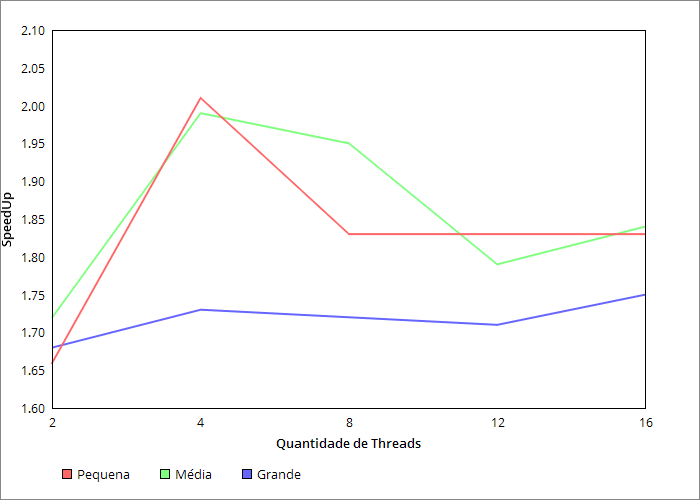
\includegraphics[scale=0.35]{speedup.png}
      \caption{SpeedUp pela quantidade de threads dos experimentos inicialmente realizados, cada linha representando um tamanho de entrada diferente, sendo estas Pequena: 500M; Média: 1GB e Grande: 2GB.}
      \label{figurelabel}
   \end{figure}
De fato, ao isolarmos as entradas \textit{Pequena} e \textit{Média}, verificamos que a média de \textit{speedup} desta ($1.882$) foi melhor se comparada àquela ($1.892$). Em detrimento da quantidade superior de dados, o \textit{speedup} da entrada \textit{Média} deveria e realmente se sobressaiu. Por outro lado, pela entrada \textit{Grande} possuir o maior tamanho dentre as três, esperava-se que também possuísse o maior \textit{speedup}. Conforme à Figura 1, obviamente não foi o caso.

Tendo isto em vista, investigamos fatores que poderiam influenciar no tempo de execução dos programas paralelos. A Figura 2 indica o \textit{speedup} de uma entrada intermediaria entre às entrada \textit{Média} e \textit{Grande} que nomearemos \textit{turning point}. Mediante à Figura, obtemos o resultado esperado, ou seja, conforme o tamanho da entrada intermediaria aumentou, a média de \textit{speedup} cresceu, sendo: $2.268$ contraposta a $1.892$.
\begin{figure}[thpb]
      \centering
      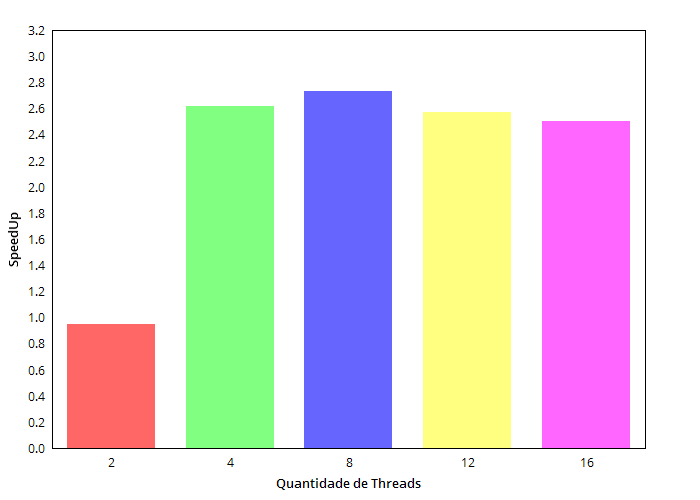
\includegraphics[scale=0.35]{speedup1.8.png}
      \caption{ Speedup pela quantidade de threads para a entrada 1.8 GB}
      \label{figurelabel2}
   \end{figure}

Como mencionado na seção II.C, o \textit{swap} é um dos fatores relacionados ao \textit{hardware} que poderia influenciar na análise da taxa \textit{speedup}. O \textit{swap} em relação à cada entrada por \textit{thread} é apresentado na Figura 3. Na Figura, verifica-se que as entradas \textit{Pequena} e \textit{Média} não formam afetadas pelo tempo de \textit{swap}. Por outro lado, o \textit{turning point} assim como a maior entrada foram impactados. Destacamos, no entanto, que o \textit{turning point} teve uma média de transferência de 11MB se comparado à entrada Grande, cuja média foi 35MB, resultando em um uso 3 vezes maior e, por conseguinte, tendo uma taxa de \textit{speedup} inferior.

Embora o recurso de \textit{swap} auxilie o sistema operacional à gerenciar diversos fluxos para além do programa sendo executado, aliviando um pouco da sobrecarga da memória principal, provoca uma busca por dados em uma memória mais lenta e, consequentemente, impacta no tempo de execução do programa, ocasionando uma queda na taxa de \textit{speedup} de entradas maiores. 

\begin{figure}[thpb]
      \centering
      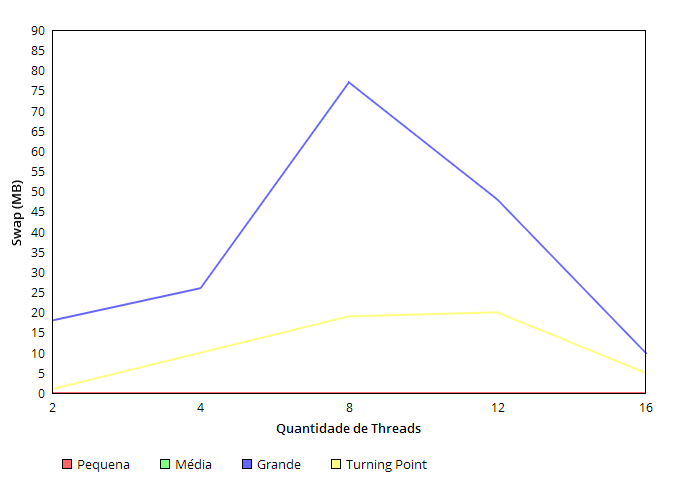
\includegraphics[scale=0.35]{swap.png}
      \caption{ Swap pela quantidade de threads das entradas Pequena, Média, Grande e Turning Point.}
      \label{figurelabel3}
   \end{figure}
   
Outro fator passível de discussão está relacionado ao pico do \textit{speedup} estando próximo ao uso de 4 \textit{threads}. O comportamento pode ser explicado por meio da quantidade de núcleos disponíveis na máquina, sendo este 4. Ao exceder esse número, os processos se tornam altamente voláteis, ocasionando muita troca de contexto para gerenciar a execução de diversos fluxos. Essa suposição pode ser corroborada por meio da Figura 4. Na Figura, verifica-se que a quantidade de troca de contexto ao paralelizar o problema utilizando 2 e 4 \textit{threads} é inferior se comparada a 8,12 e 16. 

\begin{figure}[thpb]
      \centering
      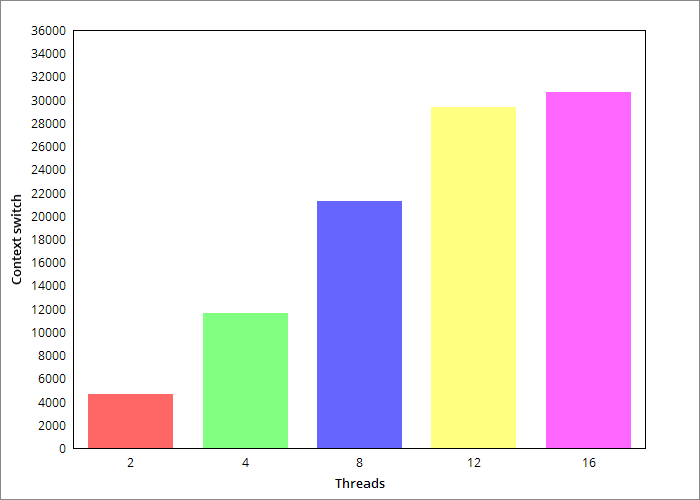
\includegraphics[scale=0.35]{cs.png}
      \caption{ Troca de contexto pela quantidade de threads da entrada Turning Point.}
      \label{figurelabel4}
   \end{figure}

\section{Conclusão}
Neste trabalho, a fim de avaliar quais são os impactos do uso paralelismo na criptografia de cifras clássicas como o \textit{Rail Fence Cipher}, realizamos um conjunto de experimentos cujo resultado possibilitou um maior entendimento acerca das vantagens do paralelismo bem como suas limitações. 

Por meio da percepção empírica e constatação teórica, acreditamos que ao utilizar o paralelismo, existe a possibilidade de exceder à performance serial, dado que seja ponderado o tamanho da entrada do programa com as especificações da máquina utilizada. 

Como verificado ao longo deste trabalho, existe um limite computacional intrinsecamente relacionado ao \textit{hardware} no âmbito do paralelismo. Sendo assim, ao adotar a estratégia cujo enfoque seja distribuir processamento entre \textit{threads}, é importante conhecer os limites da memória principal, a fim de evitar troca de informações desnecessária com o disco rígido durante a execução do programa. Bem como alternar o números de threads, tendo vista que, em detrimento do \textit{overhead}, é preciso encontrar uma quantidade ideal, pois nem sempre um maior número implicará em resultados melhores.

Para trabalhos futuros, pretende-se investigar outras métricas que poderiam ser exploradas para a avaliação de performance do paralelismo, assim como realizar outros estudos de caso, englobando problemas que tenha maior dependência entre os dados, para investigar se o uso de paralelismo ainda proporciona resultados interessantes mesmo com forte dependência entre os processos. 

Além disso, durante os experimentos, foi constatado que ao passo que o número de \textit{threads} excedia o número de núcleos disponíveis pela máquina (4) e o tamanho da entrada de dados fosse superior ao limite da memória, o \textit{speedup} foi fortemente prejudicado. Com isso, pretende-se realizar experimentos em máquinas que possuem melhores recursos computacionais para obtermos resultados mais significantes.



\begin{thebibliography}{99}

\bibitem{c1} Peter Pacheco. 2011. An Introduction to Parallel Programming (1st. ed.). Morgan Kaufmann Publishers Inc., San Francisco, CA, USA.

\bibitem{c2}Krothapalli, V. Prasad, and P. Sadayappan. "An approach to synchronization for parallel computing." Proceedings of the 2nd international conference on Supercomputing. 1988.

\bibitem{c3}Gioiosa, Roberto, et al. "Analysis of system overhead on parallel computers." Proceedings of the Fourth IEEE International Symposium on Signal Processing and Information Technology, 2004..

\bibitem{c4}Apostolico, Alberto, et al. "Efficient parallel algorithms for string editing and related problems." SIAM Journal on Computing 19.5 (1990): 968-988.

\bibitem{c5}Wood, David A., and Mark D. Hill. "Cost-effective parallel computing." Computer 28.2 (1995): 69-72.

\bibitem{c6}Theis, Thomas N., and H-S. Philip Wong. "The end of moore's law: A new beginning for information technology." Computing in Science \& Engineering 19.2 (2017): 41-50.

\bibitem{c7}Qasem, Mais Haj, and Mohammad Qatawneh. "Parallel Hill Cipher Encryption Algorithm." International Journal of Computer Applications 179.19 (2018): 16-24.

\bibitem{c8}Fox,  Geoffrey  C.,  Steve  W.  Otto,  and  Anthony  JG  Hey. "Matrix     algorithms     on     a     hypercube     I:     Matrix multiplication." Parallel computing 4.1 (1987): 17-31.

\bibitem{c9}Cannon, Lynn E. A Cellular Computer to Implement the Kalman  Filter  Algorithm.  No.  603-Tl-0769.  Montana State Univ Bozeman Engineering Research Labs, 1969.

\bibitem{c10}Panigrahy, S. K., Acharya, B., \& Jena, D. (2008). Image encryption  using  self-invertible  key  matrix  of  hill  cipher algorithm.
\end{thebibliography}





\end{document}
